\begin{figure}[H]
\centering
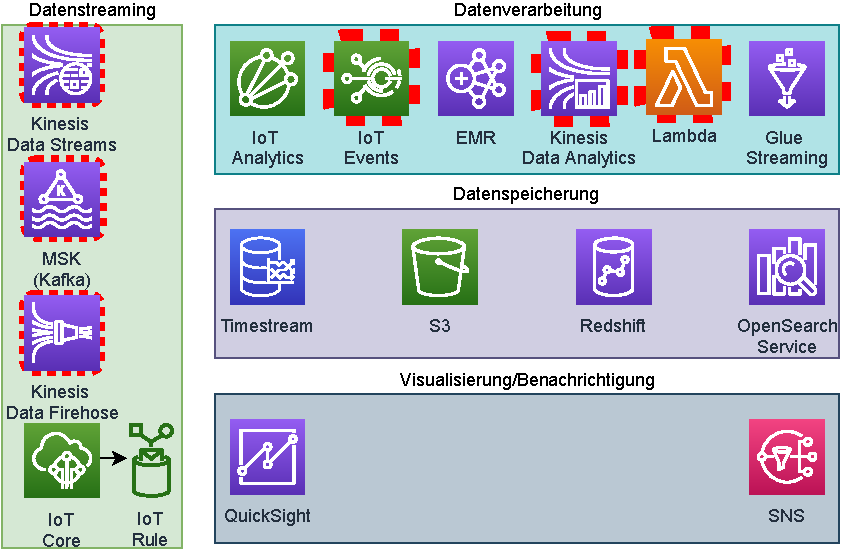
\includegraphics[width=\textwidth]{graphics/Overview-Realtime.pdf}
\caption{Einsetzbare Produkte im Bereich Echtzeitverarbeitung}
\label{abb:ProdukteRT}
\end{figure}


===========

Innerhalb des \ac{IoT} Core Brokers ist es möglich, Regeln zu definieren, die einzelne Nachrichten aus Topics in andere Dienste weiterzuleiten. Dazu müssen besagte Nachrichten selektiert werden, was mittels eines SQL Dialekts möglich ist. Eine beispielhafte Selektion könnte folgendermaßen aussehen: 


\begin{figure}[H]
\centering
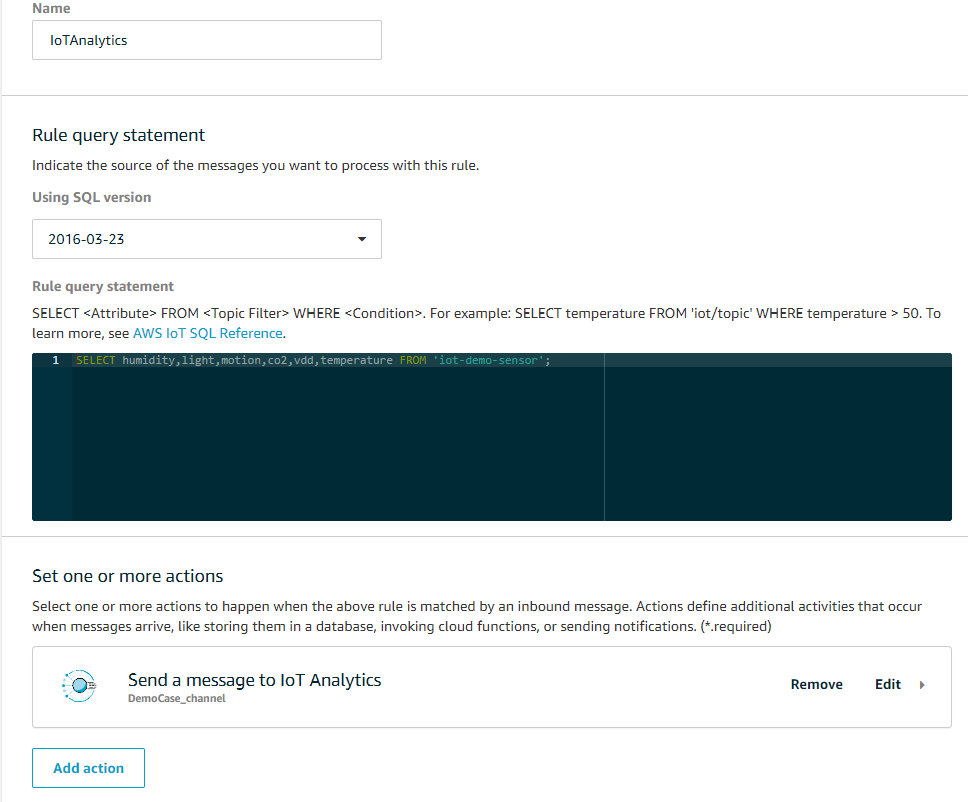
\includegraphics[width=\textwidth]{graphics/IoT-Rules-console.png}
\caption{Einstellung einer neuen Regel zur Weiterleitung an IoT Analytics}
\label{abb:IoTRulesExample}
\end{figure}

In \autoref{abb:IoTRulesExample} ist die Erstellung einer Weiterleitungsregel mit folgendem SQL Code zu sehen:
\lstset{language=SQL} 
\begin{lstlisting}
SELECT humidity,light,motion,co2,vdd,temperature 
FROM 'iot-demo-sensor'
\end{lstlisting}
Die Nachrichten aus dem Topic iot-demo-sensor werden dabei beispielhaft an IoT Analytics weitergeleitet.

\subsection{AWS IoT Analytics} \label{productselection:iotanalytics}
\AWSIOT Analytics ist ein Dienst der \AWSIOT Produktfamilie, der nach Aussage des Herstellers weitreichende Analysen von \ac{IoT} Daten, die beispielsweise via \AWSIOT Core geladen werden können, zulässt.
\begin{figure}[H]
\centering
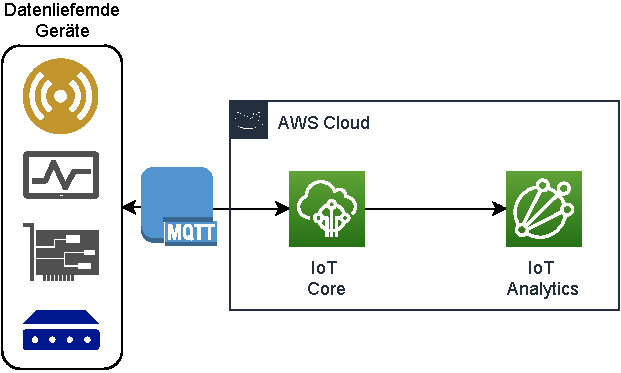
\includegraphics[width=0.8\textwidth]{graphics/IoT-Analytics-general.pdf}
\caption{Grobarchitektur des Ablaufes für IoT Analytics}
\label{abb:GrobArchitekturIoTAnalytics}
\end{figure}
In \autoref{abb:GrobArchitekturIoTAnalytics} ist die Grobarchitektur und Verknüpfung mit anderen Diensten unter Annahme der Vorraussetzungen aus \autoref{chap:rahmendatenverarbeitung} gezeigt. Datenliefernde Geräte, wie beispielsweise Sensoren liefern Zeitreihen-Messwerte via dem \ac{MQTT} Protokoll an. Die Weiterleitung zu IoT Analytics erfolgt mittels einer eingerichteten Regel im \ac{IoT} Core Messagebroker, welche mittels eines Dialekts der SQL Sprache gewisse Topics vorselektiert oder alle Topics zulässt.

\subsection{AWS IoT Events}

\begin{figure}[H]
\centering
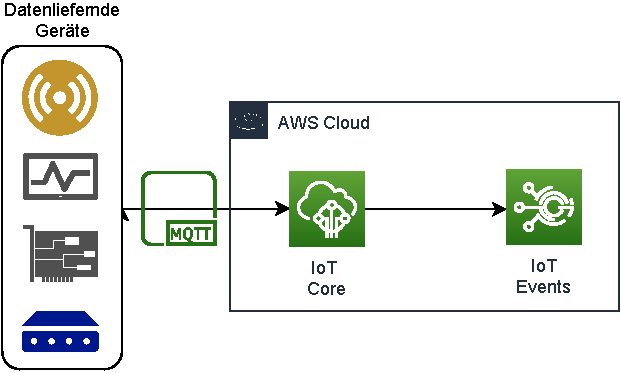
\includegraphics[width=0.8\textwidth]{graphics/IoT-Events-general.pdf}
\caption{Grobarchitektur des Ablaufes für IoT Events}
\label{abb:GrobArchitekturIoTEvents}
\end{figure}

\Todo{IoT Events ansprechen (Schwellwerte)}

\subsection{Amazon Kinesis}
Amazon Kinesis ist im Gegensatz zu \AWSIOT Analytics nicht allein auf die Analyse von \ac{IoT} Daten spezialisiert. Kinesis eignet sich vielmehr für generelle Analysen von allerlei Streamingdaten. Zusätzlich ist Amazon Kinesis älter als \AWSIOT Analytics.

\begin{figure}[H]
\centering
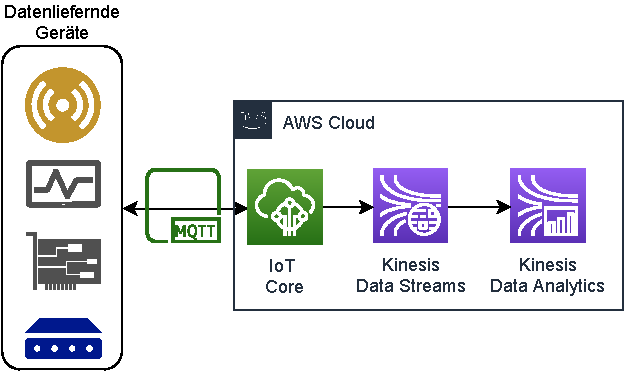
\includegraphics[width=0.8\textwidth]{graphics/Kinesis-Analytics-general.pdf}
\caption{Grobarchitektur des Ablaufes für Kinesis Analytics}
\label{abb:GrobArchitekturKinesisAnalytics}
\end{figure}
In \autoref{abb:GrobArchitekturKinesisAnalytics} ist das Zusammenspiel der Dienste aus der Kinesis Familie mit anderen Diensten dargestellt. Angenommen werden dabei die in \autoref{chap:rahmendatenverarbeitung} erläuterten Rahmenbedingungen, weshalb \ac{IoT} Core als Message Broker eingesetzt ist. Wie in der in \autoref{productselection:iotanalytics} beschriebenen Architektur, muss auch hier für die Datenverarbeitung eine Regel im \ac{IoT} Core Broker angelegt werden, um relevante Nachrichten an Kinesis Data Streams weiterzuleiten.\footcite[Vgl.][]{AmazonWebServicesInc..o.J.}

\begin{figure}[H]
\centering
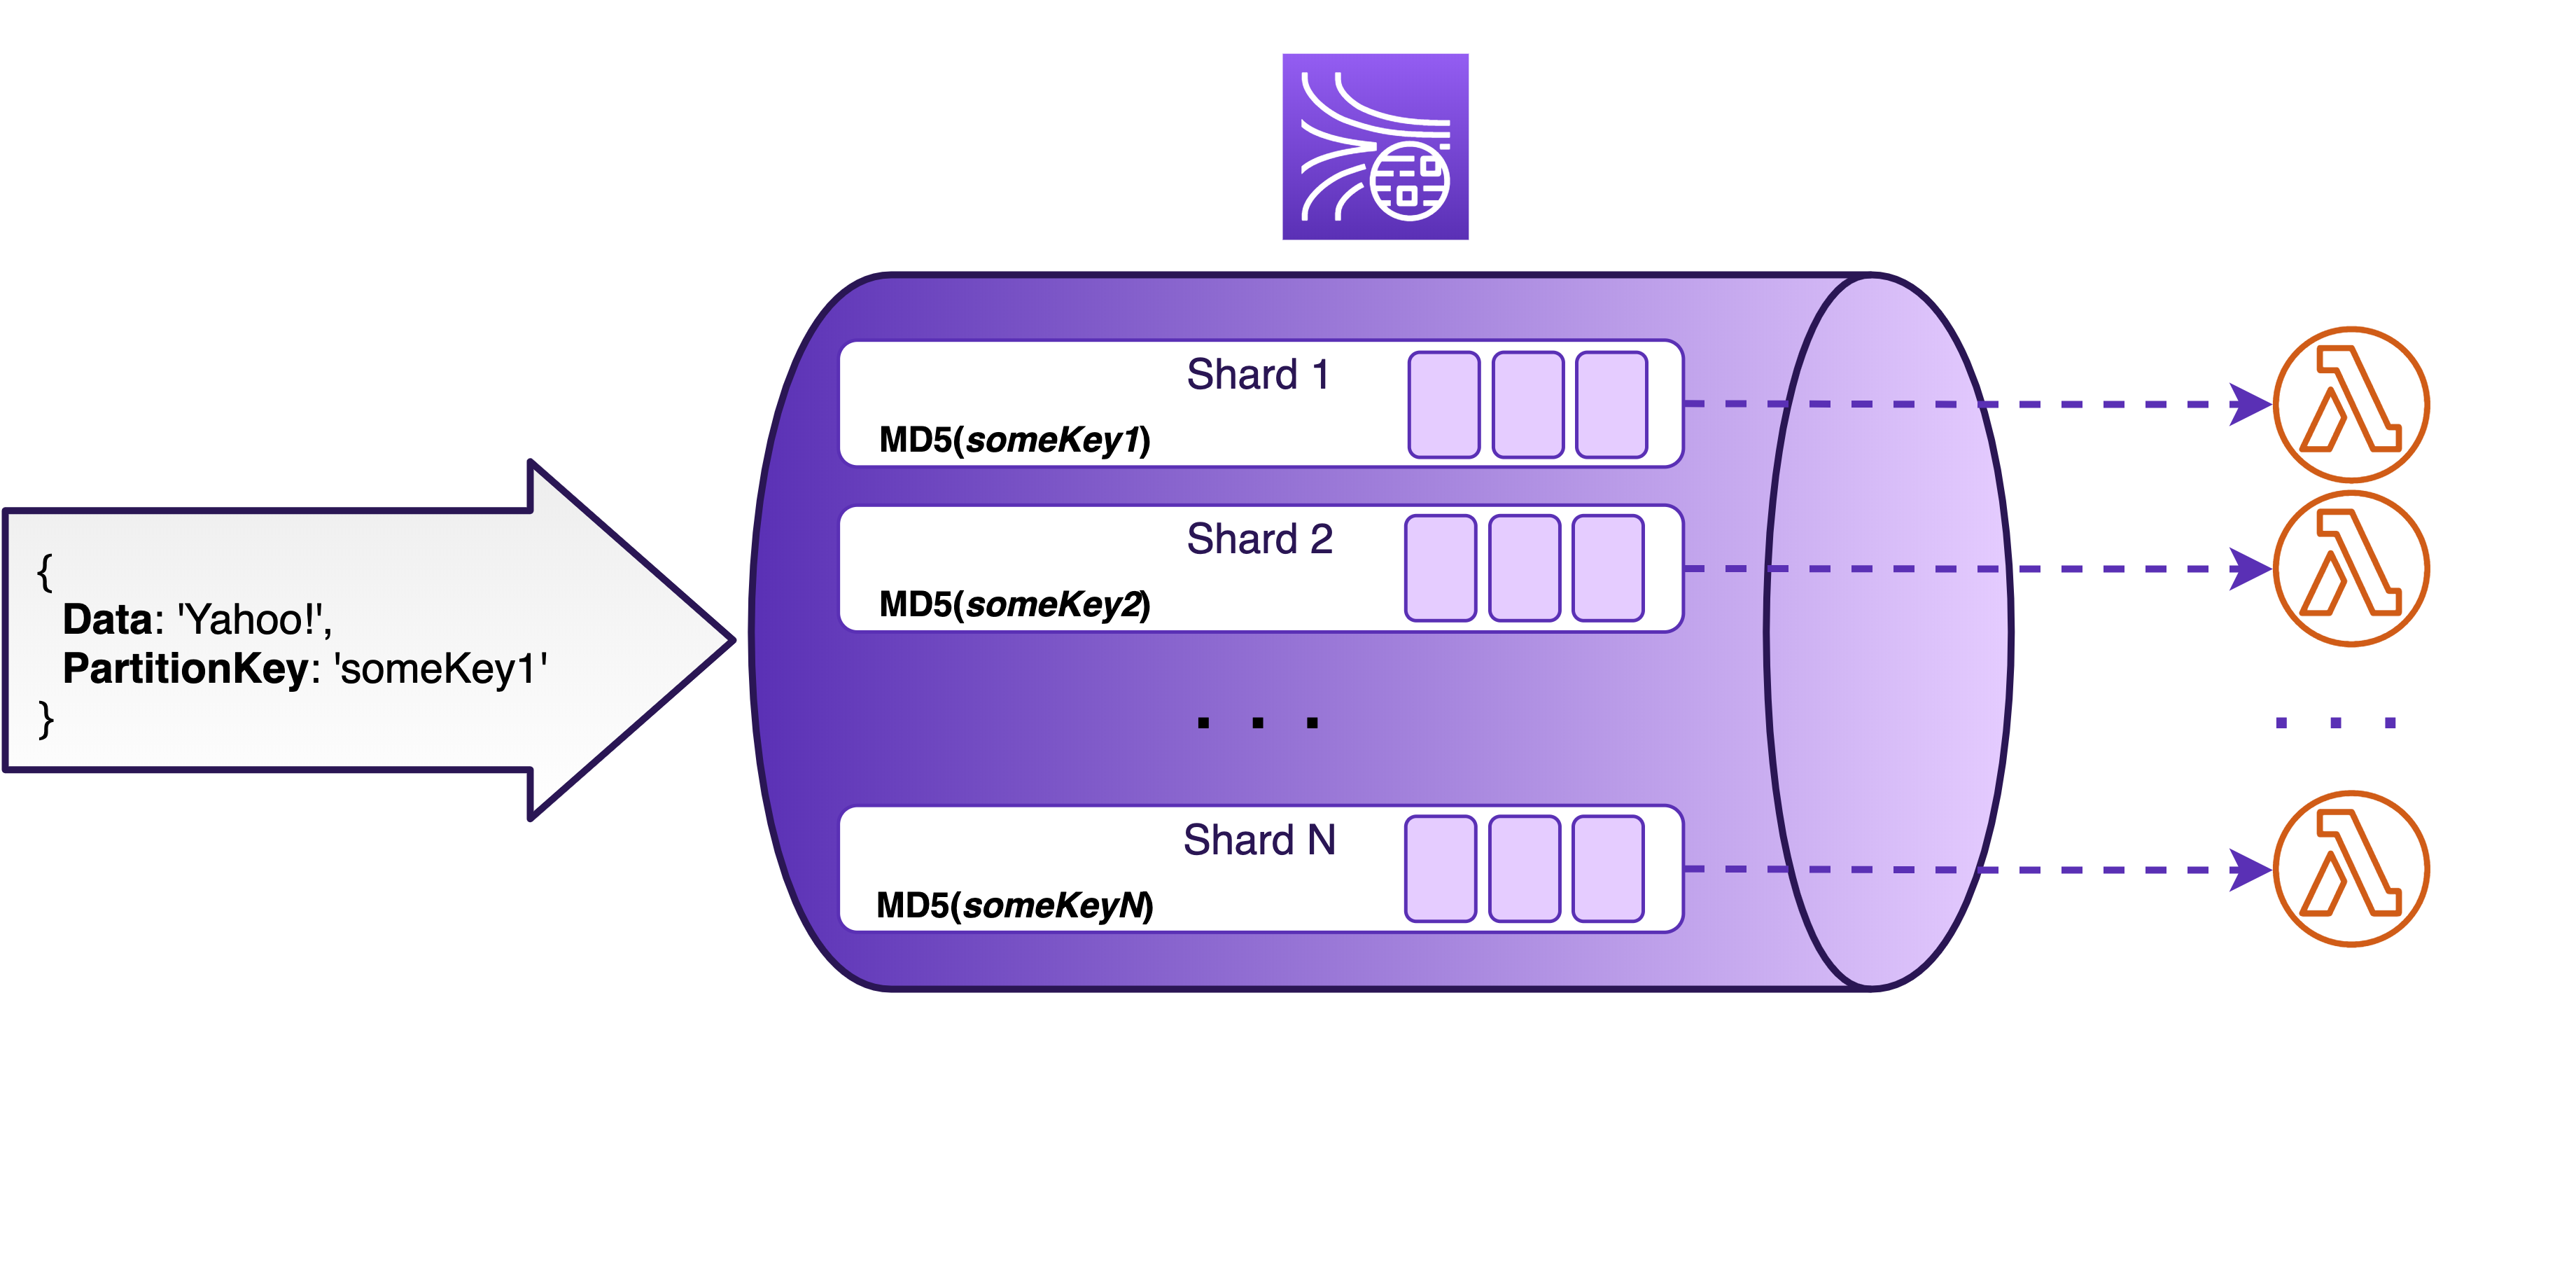
\includegraphics[width=\textwidth]{graphics/kinesis-inner-workings.png}
\caption[Funktionsweise von Kinesis]{Funktionsweise von Kinesis.\footnotemark}
\label{abb:KinesisShards}
\end{figure}
\footnotetext{Entnommen aus: \cite{Pogosova.28.05.2020}}
Kinesis unterteilt, wie in \autoref{abb:KinesisShards} gezeigt, Daten in einzelne Partitionen/Shards, in denen gleich partitionierte Datensätze verarbeitet werden können.\footcite[Vgl. auch im Folgenden][]{Pogosova.28.05.2020} Einzelne Shards verhalten sich dabei wie geordnete Warteschlangen und speichern die Nachrichten nach Eingangsdatum sortiert. 


\subsection{AWS Lambda}
Bei \ac{AWS} Lambda handelt es sich um die Amazon Implementierung eines \ac{FaaS} Dienstes. Innerhalb dieser Arbeit wird Lambda als einzige generelle Computing Plattform betrachtet, da Alternativen wie \ac{EC2}, welches virtuelle Maschinen anbietet oder \ac{ECS}, welches Container anbietet einen von einzelnen Events unabhängigen Lebenszyklus haben. So laufen Container auf \ac{ECS} oder virtuelle Maschinen auf \ac{EC2}, wenn nicht anders konfiguriert kontinuierlich und holen/ \enquote{fetchen} Daten. In Zeiträumen, in denen keine Daten bereitstehen sind die entsprechenden Container und virtuellen Maschinen im Leerlauf, was unnötige Kosten erzeugt. Lambda hingegen wird von unterstützenden Diensten zur Verarbeitung von Events aufgerufen. Dabei ist je nach Dienst einstellbar, ob ein Aufruf pro Event stattfinden soll, oder Events zu einer konfigurierbaren Anzahl gruppiert werden und dann an Lambda übergeben werden. Lambda eignet sich besonders für analytische Workloads, seit der kürzlichen Addition von Intels \ac{AVX2}, einem speziellen CPU-Instruktionssatz, der die Verarbeitung von Vektorinstruktionen, wie sie beispielsweise beim Machine Learning oder in der Statistik vorkommen, beschleunigt.\footcite[Vgl.][]{Beswick.24.11.2020} Aufgrund der zentralen Rolle im Bereich Compute bei \ac{AWS}, können viele Dienste Events an Lambda senden. In \autoref{abb:GrobArchitekturLambda} sind als Integrationsbeispiele die \acp{MoM} \ac{IoT} Core, MQ und Kinesis Data Streams als Eventlieferanten gezeigt.
\begin{figure}[H]
\centering
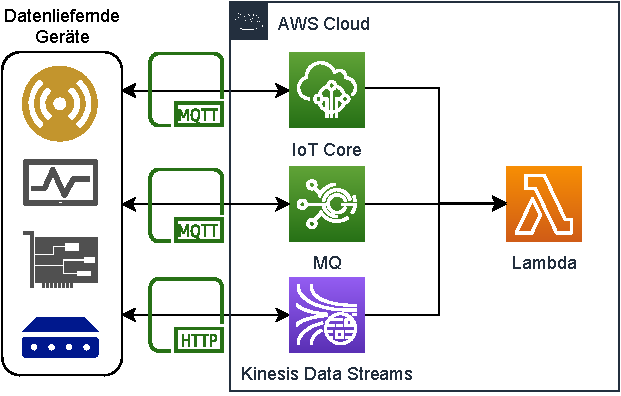
\includegraphics[width=0.8\textwidth]{graphics/Lambda-general.pdf}
\caption{Grobarchitektur des Ablaufes für Lambda}
\label{abb:GrobArchitekturLambda}
\end{figure}

\subsection{Amazon MSK}
Bei \ac{MSK} handelt es sich um einen Managed Service für die Open Source Lösung Apache Kafka. Im Gegensatz zu anderen, hier im Kapitel aufgeführten Lösungen wie \ac{IoT} Analytics, hat Amazon \ac{MSK} nicht von Grund auf selber entwickelt, sondern einen großen Teil des Codes von Apache Kafka übernommen. Dies erklärt auch, warum die Anbindung an andere Dienste von Amazon bedeutend schwieriger ist, als beispielsweise an \ac{IoT} Core. In der in \autoref{abb:GrobArchitekturMSK} abgebildeten Grobarchitektur müsste zur Anbindung von Apache Kafka an zuliefernde Geräte ein Intermediär wie \ac{IoT} Core verrwendet werden, da Apache Kafka ein eigenes, binäres Protokoll hat, welches sonst in die Geräte implementiert werden müsste. \Todo{letzten Halbsatz belegen} Umgangen kann die Implementierung des Kafka Protokolls auf dreierlei Arten: Zum einen lassen sich mittels Kafka Connect for \ac{MQTT} \ac{MQTT} Broker als Eventquellen anbinden.\footcite[Vgl.][]{Erber.12.01.2021} Alternativ kann Kafka auch als \ac{MQTT} Proxy dienen, was bedeutet, dass Kafka als eigenständiger MQTT Broker agiert, wobei zu beachten ist, dass Kafka weit nicht alle \ac{MQTT} Standardelemente implementiert und eine paralelle Weiterverarbeitung in anderen Amazon Diensten nicht möglich ist.\footcite[Vgl.][]{Erber.12.01.2021} Zuletzt gibt es noch die Möglichkeiten, die Nachrichten via \ac{IoT} Core innerhalb von \ac{AWS} an \ac{MSK} weiterzuleiten, was auch in \autoref{abb:GrobArchitekturMSK} dargestellt ist.
\begin{figure}[H]
\centering
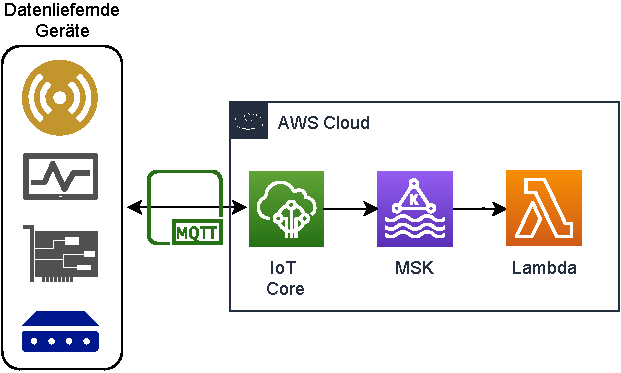
\includegraphics[width=0.8\textwidth]{graphics/MSK-general.pdf}
\caption{Grobarchitektur des Ablaufes für Managed Streaming for Apache Kafka}
\label{abb:GrobArchitekturMSK}
\end{figure}

Kafka hat eigene Verarbeitungslogiken integriert, mit welchen einige Analysen bereits durchgeführt werden können. Um diese in \ac{AWS} weiterverarbeiten zu können, müssen die Ergebnisse via der Integration mit Lambda oder der Integration mit \ac{EC2}, der Amazon Plattform für virtuelle Maschinen abgerufen werden.

=> binary protocol no \ac{MQTT} Support, redundant, only Lambda and EC2 conenctivity

\subsection{Produktauswahl}